\documentclass[aspectratio=169,11pt]{beamer}

% ============================================================
% PACKAGES
% ============================================================
\usepackage{graphicx}
\usepackage{tikz}
\usetikzlibrary{positioning,arrows.meta}
\usepackage{xcolor}
\usepackage{booktabs}
\usepackage{tabularx}
\usepackage{array}
\usepackage{ragged2e}
\usepackage{hyperref}

% ============================================================
% COLORS - SAME AS PHASE-I
% ============================================================
\definecolor{GEUBlue}{RGB}{20,55,105}
\definecolor{GEULightBlue}{RGB}{238,244,251}
\definecolor{GEUGrey}{RGB}{90,90,90}
\definecolor{GEULightGrey}{RGB}{245,246,248}

% ============================================================
% BEAMER SETTINGS
% ============================================================
\usetheme{default}
\setbeamertemplate{navigation symbols}{}
\setbeamertemplate{blocks}[rounded][shadow=false]

\setbeamercolor{normal text}{fg=black,bg=white}
\setbeamercolor{frametitle}{fg=GEUBlue}
\setbeamercolor{structure}{fg=GEUBlue}
\setbeamercolor{block title}{fg=GEUBlue,bg=GEULightBlue}
\setbeamercolor{block body}{fg=black,bg=GEULightBlue}

\setbeamerfont{frametitle}{size=\Large,series=\bfseries}

% ============================================================
% LOGO
% ============================================================
% Upload the Graphic Era logo with this filename to Overleaf.
\newcommand{\GEULogo}{graphicera_logo.png}

% ============================================================
% HEADER
% ============================================================
\setbeamertemplate{headline}{%
  \begin{tikzpicture}[remember picture,overlay]
    \node[
        anchor=north east,
        xshift=-0.30cm,
        yshift=-0.12cm
    ] at (current page.north east)
    {\includegraphics[height=0.62cm]{\GEULogo}};
  \end{tikzpicture}
  \vspace{0.72cm}
}

% ============================================================
% FRAME TITLE
% ============================================================
\setbeamertemplate{frametitle}{%
  \vspace{0.03cm}
  \insertframetitle\par
  \vspace{0.04cm}
  \textcolor{GEUBlue}{\rule{\textwidth}{0.9pt}}
  \vspace{0.03cm}
}

% ============================================================
% FOOTER
% ============================================================
\setbeamertemplate{footline}{%
  \leavevmode
  \hbox{%
  \begin{beamercolorbox}[
      wd=.82\paperwidth,
      ht=0.32cm,
      dp=0.10cm,
      leftskip=.3cm
  ]{author in head/foot}
    \tiny Department of Computer Science \& Engineering |
    Graphic Era (Deemed to be University)
  \end{beamercolorbox}%
  \begin{beamercolorbox}[
      wd=.18\paperwidth,
      ht=0.32cm,
      dp=0.10cm,
      rightskip=.3cm
  ]{date in head/foot}
    \hfill\tiny\insertframenumber/\inserttotalframenumber
  \end{beamercolorbox}}
}

% ============================================================
% CUSTOM COMMANDS
% ============================================================
\newcommand{\smallnote}[1]{%
\vspace{0.08cm}
{\scriptsize\color{GEUGrey}#1}
}

\newcommand{\placeholder}[1]{%
\textit{\color{GEUGrey}#1}
}

% ============================================================
% DOCUMENT INFORMATION
% ============================================================
\title{\textbf{Project-Based Learning}\\[2mm]\large Phase-II Evaluation}
\author{\textbf{PrioriTask: Intelligent Task Scheduling System}\\Team ID: T-315}

\institute{
Department of Computer Science \& Engineering\\
Graphic Era (Deemed to be University), Dehradun
}

\date{Academic Session 2026--27}

% ============================================================
% DOCUMENT
% ============================================================
\begin{document}

% ============================================================
% SLIDE 1
% ============================================================
\begin{frame}[plain]

\begin{tikzpicture}[remember picture,overlay]

\draw[GEUBlue,line width=3pt]
(current page.north west) -- (current page.north east);

\node[
    anchor=north east,
    xshift=-0.45cm,
    yshift=-0.35cm
] at (current page.north east)
{\includegraphics[height=1.0cm]{\GEULogo}};

\node[
    align=center,
    text width=.84\paperwidth
] at ([yshift=.25cm]current page.center)
{
{\color{GEUBlue}
\fontsize{26}{30}\selectfont
\bfseries PROJECT-BASED LEARNING}
\\[3mm]

{\fontsize{18}{22}\selectfont
PHASE-II EVALUATION}
\\[7mm]

{\color{GEUGrey}
\Large\bfseries
PrioriTask: Intelligent Task Scheduling System}
\\[2mm]

{\color{GEUBlue}
\normalsize Team ID: T-315}
};

\node[
    align=center,
    anchor=south,
    yshift=.42cm
] at (current page.south)
{
\bfseries
Department of Computer Science \& Engineering\\
Graphic Era (Deemed to be University), Dehradun\\[-1mm]
\scriptsize Academic Session 2026--27
};

\end{tikzpicture}

\end{frame}

% ============================================================
% SLIDE 2
% ============================================================
\begin{frame}{Team \& Mentor Details}

\begin{columns}[T,totalwidth=\textwidth]

\column{.48\textwidth}

\begin{block}{Team Information}
\begin{tabular}{@{}ll@{}}
\textbf{Team ID:} & T-315\\
\textbf{Semester:} & 3rd\\
\textbf{Section:} & A, ML4, CYBER\\
\textbf{Domain:} & Systems Programming /\\
                 & Scheduling Algorithms
\end{tabular}
\end{block}

\column{.48\textwidth}

\begin{block}{Team Members}
\scriptsize
1.\quad Manisha Bisht --- 2510012646\\
\\[1mm]
2.\quad Purnima --- 2510012541\\
\\[1mm]
3.\quad Yug Bhardwaj --- 2512500006\\
\end{block}

\end{columns}

\vspace{2mm}

\begin{block}{Mentor}
Dr. Hriday Kumar Gupta
\hfill
\textbf{Interactions completed: 4}
\end{block}

\vfill

\smallnote{
}

\end{frame}

% ============================================================
% SLIDE 3
% ============================================================
\begin{frame}{Phase-I Recap \& Feedback Incorporated}

\begin{block}{Phase-I Status}
\small
Phase-I proposed a C++ and SQLite task scheduler built around
\textbf{task compression}: when a day is fully busy, shrink task durations
toward a minimum instead of dropping work. Phase-I delivered the
concept, a schema sketch and the technology selection.
\end{block}

\vspace{2mm}

\begin{columns}[T,totalwidth=\textwidth]

\column{.48\textwidth}

\textbf{\color{GEUBlue}Feedback Received}

\begin{itemize}\itemsep2pt
\small
\item Correct implementation of C++ classes.
\item Addition in core idea of the project.
\item Scheduler output overwrote task definitions.
\end{itemize}

\column{.48\textwidth}

\textbf{\color{GEUBlue}Changes Incorporated}

\begin{itemize}\itemsep2pt
\small
\item \texttt{Database} class owns the SQLite connection
\item Added task-dropping, an energy-aware advisor and commitments
\item Added a separate \texttt{day\_plan} allocation table
\end{itemize}

\end{columns}

\vfill

\smallnote{
}

\end{frame}

% ============================================================
% SLIDE 4
% ============================================================
\begin{frame}{Problem Statement \& Finalized Objectives}

\begin{block}{Problem Statement}
\small
Conventional to-do applications assume the day has unlimited space to work. They sort
tasks, but when total work exceeds the hours available they have no answer except
dropping tasks. PrioriTask addresses the overbooked day: deciding \emph{how much}
of each task survives, and only then \emph{which} tasks must move.
\end{block}

\vspace{2mm}

\textbf{\color{GEUBlue}Finalized Objectives}

\begin{enumerate}\itemsep3pt
\small
\item Give every task an ideal duration and a minimum below which it loses value
\item Fit tasks into the time left today with two compression policies
\item Drop optional tasks when compression is not enough; never mandatory ones
\item Suggest the best task now from deadline, priority and energy
\end{enumerate}

\vfill


\end{frame}

% ============================================================
% SLIDE 5
% ============================================================
\begin{frame}{Updated System Architecture / Workflow}

\begin{center}

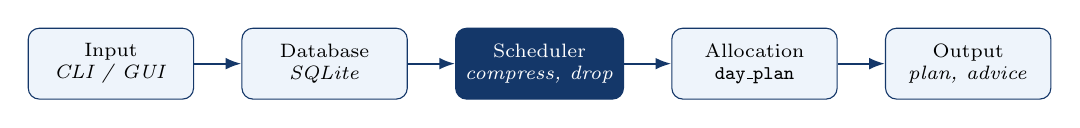
\begin{tikzpicture}[
node distance=6mm,
box/.style={
rectangle,
rounded corners,
draw=GEUBlue,
fill=GEULightBlue,
minimum width=2.10cm,
minimum height=9mm,
align=center,
font=\scriptsize
},
dark/.style={
box,
fill=GEUBlue,
text=white
},
arrow/.style={
-{Latex[length=2mm]},
thick,
draw=GEUBlue
}
]

\node[box] (a) {Input\\\textit{CLI / GUI}};
\node[box,right=of a] (b) {Database\\\textit{SQLite}};
\node[dark,right=of b] (c) {Scheduler\\\textit{compress, drop}};
\node[box,right=of c] (d) {Allocation\\\texttt{day\_plan}};
\node[box,right=of d] (e) {Output\\\textit{plan, advice}};

\draw[arrow] (a)--(b);
\draw[arrow] (b)--(c);
\draw[arrow] (c)--(d);
\draw[arrow] (d)--(e);

\end{tikzpicture}

\end{center}

\vspace{3mm}

\begin{columns}[T,totalwidth=\textwidth]

\column{.48\textwidth}

\textbf{\color{GEUBlue}Major Components}

\begin{itemize}\itemsep2pt
\scriptsize
\item \texttt{database.h} -- \texttt{Database} class wrapping the SQLite C
      API; \texttt{Task} struct reflecting one row
\item \texttt{scheduler.h/.cpp} -- compression and task-dropping, zero SQLite
      dependency
\item \texttt{main.cpp} (CLI) and \texttt{gui.cpp} (desktop GUI) -- complete
\end{itemize}

\column{.48\textwidth}

\textbf{\color{GEUBlue}Changes Since Phase-I}

\begin{itemize}\itemsep2pt
\scriptsize
\item \texttt{day\_plan} table separates scheduler output from task
      definitions
\item Scheduler fully decoupled --- compiles and tests without linking SQLite
\item Desktop GUI (Dear ImGui) and CLI share one engine
\end{itemize}

\end{columns}

\vfill


\end{frame}

% ============================================================
% SLIDE 6
% ============================================================
\begin{frame}{Module Design \& Functional Requirements}

\begin{columns}[T,totalwidth=\textwidth]

\column{.44\textwidth}

\textbf{\color{GEUBlue}Major Modules}

\begin{enumerate}\itemsep3pt
\scriptsize
\item Database / Persistence\\
      {\color{GEUGrey}\texttt{tasks}, \texttt{day\_plan}, commitments}
\item Compression Scheduler\\
      {\color{GEUGrey}two policies + task-dropping}
\item Advisor \& Commitments\\
      {\color{GEUGrey}suggestions, college / work hours}
\item Interface \& Plan Display\\
      {\color{GEUGrey}CLI and desktop GUI}
\end{enumerate}

\column{.52\textwidth}

\textbf{\color{GEUBlue}Functional Requirements}

\begin{itemize}\itemsep3pt
\scriptsize
\item Store tasks with priority, deadline, ideal and minimum duration,
      mandatory and needs-going-out flags
\item Fit the day around commitments, no task below its minimum
\item Drop optional tasks when compression is not enough; never mandatory
      ones
\item Suggest the next task; stay quiet during college hours
\end{itemize}

\end{columns}

\vfill

\begin{block}{Module Dependency}
\scriptsize
Interface $\rightarrow$ Database $\rightarrow$ Scheduler / Advisor $\rightarrow$
\texttt{day\_plan}. The logic modules are dependency-free; Database and Interface
depend on them, never the reverse --- which is what makes the algorithms
testable without a database present.
\end{block}

\end{frame}

% ============================================================
% SLIDE 7
% ============================================================
\begin{frame}{Technology Stack \& Development Methodology}

\begin{columns}[T,totalwidth=\textwidth]

\column{.48\textwidth}

\begin{block}{Technology Stack}
\scriptsize
\begin{itemize}\itemsep2pt
\item Programming: C++17
\item Database: SQLite (single-file amalgamation, compiled in)
\item Compiler: g++ 15.2 on Ubuntu (WSL)
\item Development Tools: VS Code, DB Browser for SQLite
\item GUI Toolkit: Dear ImGui 1.91.6 with GLFW and OpenGL 3
\item Version Control: Git / GitHub
\end{itemize}
\end{block}

\column{.48\textwidth}

\begin{block}{Development Methodology}
\scriptsize
\begin{enumerate}\itemsep2pt
\item Requirement Analysis \hfill {\color{GEUGrey}complete}
\item System Design \hfill {\color{GEUGrey}complete}
\item Module Development \hfill {\color{GEUGrey}complete}
\item Integration \hfill {\color{GEUGrey}complete}
\item Testing \& Validation \hfill {\color{GEUGrey}ongoing}
\end{enumerate}
\end{block}

\end{columns}

\vfill


\end{frame}

% ============================================================
% SLIDE 8
% ============================================================
\begin{frame}{Implementation of PBL Course Concepts}

\scriptsize

\begin{center}

\renewcommand{\arraystretch}{1.25}

\begin{tabularx}{.96\textwidth}
{@{}>{\bfseries}p{2.6cm}X p{2.6cm}@{}}

\toprule
Course & Concepts Actually Implemented & Project Module\\
\midrule

Data Structures in C &
\texttt{std::priority\_queue}; sorting and interval merging &
Scheduler, Advisor\\

OOPs with C++ &
\texttt{Database} class encapsulating the SQLite handle; \texttt{Task},
\texttt{ShrinkItem}, \texttt{PlanResult} structs &
Persistence + Scheduler\\

\midrule

Operating Systems &
Allocation of a fixed resource under contention --- equal versus
priority-weighted distribution, an analogue of CPU-time policy &
Scheduler\\

DBMS &
Four tables; foreign key, CHECK, UNIQUE constraints; transactions &
Database\\

\bottomrule

\end{tabularx}

\end{center}

\vfill

\begin{center}
\colorbox{GEULightBlue}{
\parbox{.88\textwidth}{
\centering
\textbf{Stated honestly:}
the Operating Systems row is an analogue, not an OS-level implementation.
Only concepts present in the code are listed.
}}
\end{center}

\smallnote{
Brief Discussion: Each concept maps to a specific source file.
}

\end{frame}

% ============================================================
% SLIDE 9
% ============================================================
\begin{frame}{Development \& Implementation Progress}

\scriptsize

\begin{center}

\renewcommand{\arraystretch}{1.25}

\begin{tabularx}{.96\textwidth}
{@{}p{3.2cm}p{1.9cm}X@{}}

\toprule
\textbf{Module} &
\textbf{Status} &
\textbf{Work Completed}\\
\midrule

Database / Persistence &
Completed &
Four tables, transactions, migration of older databases\\

Compression Scheduler &
Completed &
Both policies; all minimums respected\\

Advisor and commitments &
Completed &
Energy-based suggestions; college / work hours\\

Interface + \texttt{day\_plan} write-back &
Completed &
11-option CLI, 4-tab desktop GUI, plans saved\\

Task-dropping / priority queue &
Completed &
Drops least valuable optional tasks first\\

\bottomrule

\end{tabularx}

\end{center}

\vspace{3mm}

\begin{center}
\colorbox{GEULightBlue}{
\parbox{.78\textwidth}{
\centering
\textbf{Overall Project Completion: about 80\%} ---
13 of 16 deliverables complete, 1 in progress, 2 pending
}}
\end{center}

\vfill

\smallnote{
Brief Discussion: Remaining: routines, start times, CMake build.
}

\end{frame}

% ============================================================
% SLIDE 10
% ============================================================
\begin{frame}{Working Prototype / Demonstration}

\begin{columns}[T,totalwidth=\textwidth]

\column{.45\textwidth}

\textbf{\color{GEUBlue}Implemented Features}

\begin{itemize}\itemsep3pt
\scriptsize
\item What now: best task right now, with reasons
\item Plan my day: shrinks, then drops, to fit the day
\item Free-slot mode: quiet during college hours
\item Tasks and weekly commitments: add, edit, delete
\item Same engine behind the CLI and the GUI
\end{itemize}

\column{.51\textwidth}

\begin{block}{Prototype / Output}

\centering
\vspace{6mm}

\includegraphics[width=.48\linewidth]{whatnow.png}\hfill
\includegraphics[width=.48\linewidth]{planday.png}

\vspace{6mm}

\end{block}

\end{columns}

\vfill

\smallnote{
Brief Discussion: Live demo --- add a task, Plan my day, then What now.
}

\end{frame}

% ============================================================
% SLIDE 11
% ============================================================
\begin{frame}{Testing, Results \& Validation}

\scriptsize

\begin{center}

\renewcommand{\arraystretch}{1.3}

\begin{tabularx}{.96\textwidth}
{@{}p{2.6cm}X X p{1.0cm}@{}}

\toprule
Test / Scenario &
Expected Result &
Observed Result &
Status\\
\midrule

Compression, 4 budgets &
Matches hand computation &
Exact match; 500 min short by 85 &
Pass\\

Policy (700 min) &
Weighted protects priority 5 &
Loses 3 min versus 6 &
Pass\\

Task-dropping &
Mandatory never dropped &
All 10 checks pass &
Pass\\

Commitments &
Overlaps merged correctly &
All 37 checks pass &
Pass\\

CLI versus GUI &
Same plan in both &
62, 30, 422, 31 min &
Pass\\

\bottomrule

\end{tabularx}

\end{center}

\vspace{2mm}

\begin{block}{Results / Validation}
\scriptsize
Values computed by hand first. \textbf{Key finding:} at severe overload both policies converge.
\end{block}

\smallnote{
Brief Discussion: This finding led to task-dropping, now built.
}

\end{frame}

% ============================================================
% SLIDE 12
% ============================================================
\begin{frame}{GitHub Repository \& Development Activity}

\begin{columns}[T,totalwidth=\textwidth]

\column{.46\textwidth}

\textbf{\color{GEUBlue}Repository Information}

\begin{itemize}\itemsep3pt
\scriptsize
\item GitHub Link: github.com/manishabishtsht/Prioritask
\item Branch: main
\item README.md: present, to be expanded
\item Contributors: \placeholder{names as shown on GitHub}
\item Repository Status: active
\end{itemize}

\column{.50\textwidth}

\textbf{\color{GEUBlue}Version Control Practice}

\begin{enumerate}\itemsep3pt
\scriptsize
\item Shared repository on GitHub, branch \texttt{main}
\item \texttt{.gitignore} excluding \texttt{*.exe}, \texttt{*.o},
      \texttt{*.db}
\item Separate commit per component, with meaningful messages
\item Dear ImGui kept in \texttt{third\_party/}
\item Each member commits from their own account
\end{enumerate}

\end{columns}

\vfill



\end{frame}

% ============================================================
% SLIDE 13
% ============================================================
\begin{frame}{Individual Contribution}

\scriptsize

\begin{center}

\renewcommand{\arraystretch}{1.35}

\begin{tabularx}{.96\textwidth}
{@{}p{2.4cm}p{2.0cm}X p{1.3cm}@{}}

\toprule
Member &
Role &
Technical Contribution &
GitHub Commits\\
\midrule

Purnima &
Database lead &
Designed the \texttt{tasks} and \texttt{day\_plan} schema with foreign key
and CHECK constraints; implemented the \texttt{Database} class and NULL-safe
column reads &
\placeholder{XX}\\

Yug Bhardwaj &
Algorithms lead &
Implemented equal-split and priority-weighted compression, including
redistribution on floor contact and the termination guard &
\placeholder{XX}\\

Manisha Bisht &
Testing \& interface lead &
Built the four-budget test harness and invariant assertions; SQLite
amalgamation integration and build configuration &
\placeholder{XX}\\

\bottomrule

\end{tabularx}

\end{center}

\vspace{3mm}


\end{frame}

% ============================================================
% SLIDE 14
% ============================================================
\begin{frame}{Challenges, Remaining Work \& Phase-III Roadmap}

\begin{columns}[T,totalwidth=\textwidth]

\column{.48\textwidth}

\textbf{\color{GEUBlue}Challenges Faced}

\begin{itemize}\itemsep2pt
\scriptsize
\item Original design could not record how far a task can shrink
\item No single shrink rule fits gym ($-33\%$) and sleep ($-4.4\%$)
\item Antivirus blocked Windows builds; WSL clock ran in UTC
\end{itemize}

\vspace{1mm}

\textbf{\color{GEUBlue}Solutions / Learning}

\begin{itemize}\itemsep
\scriptsize
\item Added \texttt{min\_time} and \texttt{is\_mandatory} before any scheduling
      code was written, avoiding a later migration
\item Treated the rule as a policy choice; built and compared two
\item Moved builds to Ubuntu (WSL); set the Indian time zone
\end{itemize}

\column{.48\textwidth}

\textbf{\color{GEUBlue}Phase-III Roadmap}

\begin{enumerate}\itemsep
\scriptsize
\item Separate routines from tasks; add \texttt{fixed\_start}
\item Assign start times to planned tasks
\item Plan only tasks due soon
\item Compare greedy dropping with optimal 0/1 knapsack
\item CMake build, README with screenshots
\end{enumerate}

\end{columns}

\vfill


\end{frame}

% ============================================================
% SLIDE 15
% ============================================================
\begin{frame}{Expected Outcomes \& References}

\begin{columns}[T,totalwidth=\textwidth]

\column{.47\textwidth}

\textbf{\color{GEUBlue}Expected Final Outcomes}

\begin{itemize}\itemsep
\scriptsize
\item A desktop and CLI app that plans the day around fixed commitments
\item A compression engine with two policies, plus task-dropping
\item A schema preserving both task defaults and a history of how
 heavily each day was compressed
\end{itemize}

\column{.47\textwidth}

\textbf{\color{GEUBlue}References}

\begin{enumerate}\itemsep3pt
\scriptsize
\item SQLite Documentation, official project documentation, sqlite.org
\item ISO/IEC 14882:2017 --- Programming Languages: C++ (C++17 standard)
\item T. H. Cormen et al., \emph{Introduction to Algorithms}, MIT Press, 2009
\item Dear ImGui, github.com/ocornut/imgui
\item GLFW Documentation, glfw.org
\end{enumerate}

\vspace{2mm}

\begin{center}

\colorbox{GEUBlue}{
\parbox{.78\textwidth}{
\centering
\color{white}
\textbf{Thank You}\\
Questions \& Suggestions
}}

\end{center}

\end{columns}

\vfill


\end{frame}

\end{document}
